\documentclass{article}
\usepackage[final]{nips_2017}
\usepackage{polski}
\usepackage[utf8]{inputenc}    % allow utf-8 input
\usepackage[T1]{fontenc}       % use 8-bit T1 fonts
\usepackage{hyperref}          % hyperlinks
\usepackage{url}               % simple URL typesetting
\usepackage{booktabs}          % professional-quality tables
\usepackage{amsfonts}          % blackboard math symbols
\usepackage{nicefrac}          % compact symbols for 1/2, etc.
\usepackage{microtype}         % microtypography
\usepackage[section]{placeins} % figures kept in sections
\usepackage{graphicx}          % images
\graphicspath{ {./img/} }
\usepackage{multirow}
\usepackage{float}             % figures in place
\usepackage{caption}		   % smaller margin after figure

\renewcommand{\figurename}{Wykres}
\setlength{\belowcaptionskip}{-20pt}

\title{  Sieć konwolucyjna\\Sieci Neuronowe 2020 }

\author{
  Jakub Ciszek \\
  238035\\
}

\begin{document}

\maketitle

\newpage
\tableofcontents
\newpage

Cały kod wykorzystany w zadaniu znajduje się pod adresem: \url{https://github.com/Greenpp/sieci-neuronowe-pwr-2020}

\section{Opis badań}
\subsection{Plan eksperymentów}

Wszystkie eksperymenty zostały przeprowadzone 10 razy. Losowość przy inicjalizacji wag oraz generacji danych nie została narzucona żadnym ziarnem. Podczas badań przyjęto górną granicę 5 epok, po przekroczeniu której, uczenie zostawało przerywane. Ze względu na charakter zadania (klasyfikacja) na ostatniej warstwie użyto funkcji Softmax, a za funkcję straty przyjęto Entropię krzyżową. Użyta sieć składała się z warstwy konwolucyjnej, max pool, oraz w pełni połączonej ze 128 neuronami. Wagi były inicjalizowane metodą He, a uczenie przebiegało przy pomocy metody Adam. Jako funkcję aktywacji przyjęto ReLU.
TODO model MLP
Z powodów wydajnościowych testowanie modelu przeprowadzano co każde 32 paczki, z których każda składała się z 32 przykładów.\\
Zgodnie z instrukcją zostały przeprowadzone następujące badania:
\begin{itemize}
	\item Wpływ wielkości filtra na przebieg procesu uczenia
	\item Porównanie z MLP    
\end{itemize}
Podczas wizualizacji funkcji straty pominięto pierwsze 10 pomiarów dla lepszej czytelności.

\subsection{Charakterystyka zbiorów danych}

Danymi użytymi w zadaniu jest zbiór ręcznie pisanych cyfr \(0-9\) - MNIST. Na zbiór składa się 70,000 obrazów wielkości 28x28 pikseli. Na wyjściu znajduje się 10 klasom na wyjściu. Użyta w zadaniu wersja została podzielona na 3 zbiory:
\begin{itemize}
	\item Uczący - 50,000 przykładów.
	\item Walidujący - 10,000 przykładów.
	\item Testowy - 10,000 przykładów.
\end{itemize}
W trakcie eksperymentów wykorzystano jedynie zbiory uczący i testowy.

\newpage
\section{Eksperymenty}

\subsection{Wpływ wielkości filtra na przebieg procesu uczenia}
\subsubsection*{Założenia}

Zmienną w tym eksperymencie była wielkość filtra, przyjmowała wartości ze zbioru \(\{$3, 5, 7$\}\)
\subsubsection*{Przebieg}

Podczas eksperymentu model został zainicjalizowany 10 razy dla każdej z badanych wartości oraz wyuczony, uzyskane wyniki zostały zapisane w postaci pliku .plk do dalszej analizy.

\subsubsection*{Wyniki}
\begin{figure}[H]
	\centering
	\caption{Dokładność modelu w zależności od wielkości filtra}
	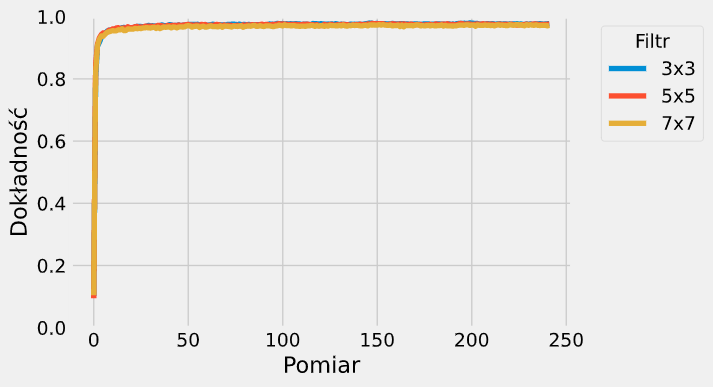
\includegraphics[width=\textwidth]{kernel_acc.png}
	\label{fig:res11}
\end{figure}
\begin{figure}[H]
	\centering
	\caption{Dokładność modelu w końcowym etapie uczenia w zależności od wielkości filtra}
	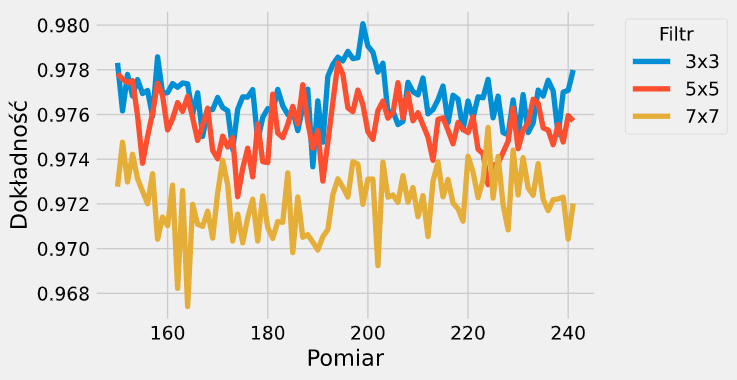
\includegraphics[width=\textwidth]{kernel_acc_zoom.png}
	\label{fig:res12}
\end{figure}
\begin{figure}[H]
	\centering
	\caption{Zachowanie funkcji błędu dla filtra wielkości 3}
	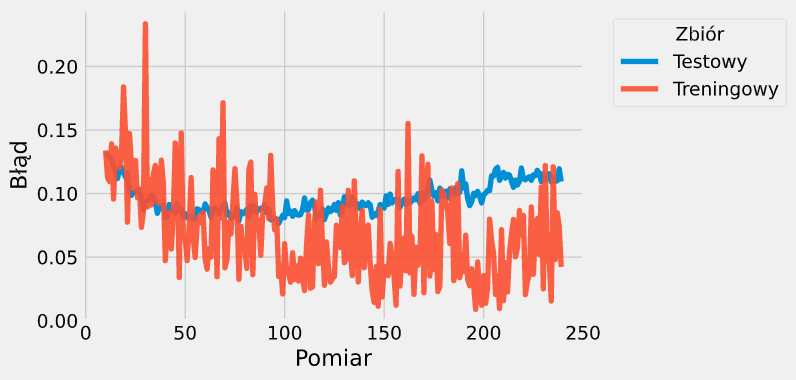
\includegraphics[width=\textwidth]{kernel_err_3.png}
	\label{fig:res13}
\end{figure}
\begin{figure}[H]
	\centering
	\caption{Zachowanie funkcji błędu dla filtra wielkości 5}
	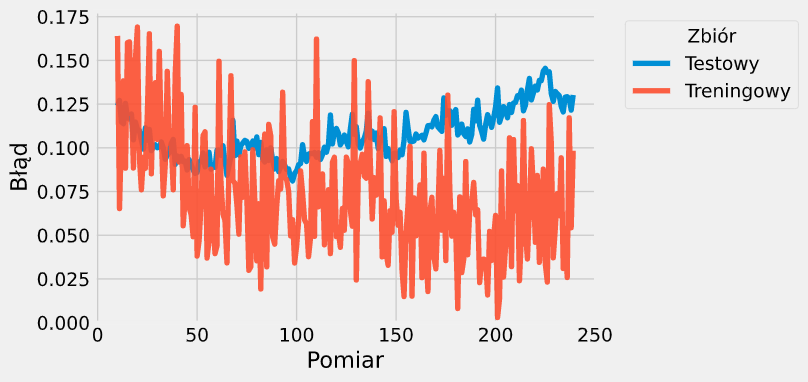
\includegraphics[width=\textwidth]{kernel_err_5.png}
	\label{fig:res14}
\end{figure}
\begin{figure}[H]
	\centering
	\caption{Zachowanie funkcji błędu dla filtra wielkości 7}
	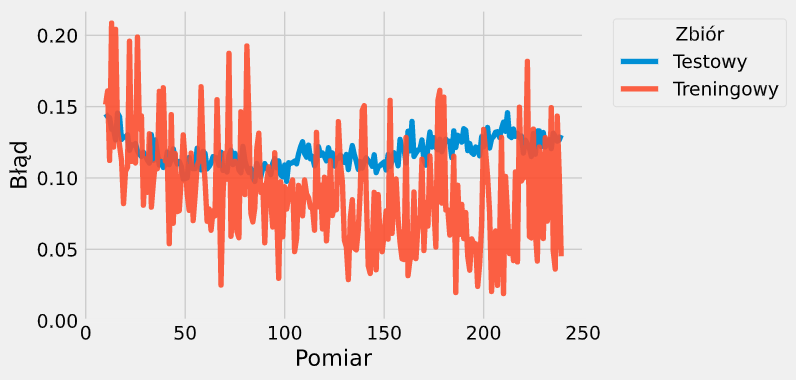
\includegraphics[width=\textwidth]{kernel_err_7.png}
	\label{fig:res15}
\end{figure}

\begin{table}[H]
	\caption{Średnia maksymalna dokładność w zależności od wielkości filtra}
	\label{tabela-res-11}
	\centering
	\begin{tabular}{rrr}
		\toprule
		Wielkość filtra & Dokładność [\%] \\
		\midrule
		3                 & \textbf{98.25}     \\
		5                 & 98.16              \\
		7                 & 97.88              \\
		\bottomrule
	\end{tabular}
\end{table}

\subsubsection*{Wnioski}

Na przedstawionych wykresach~\ref{fig:res11},~\ref{fig:res12} oraz tabeli~\ref{tabela-res-11} widać, że wielkość filtra nie ma znacznego wpływu na osiągnięty wynik. Powodem takich rezultatów może być mały rozmiar istotnych cech wyuczanych przez filtry, co mogło by powodować zbieranie dodatkowych nieistotnych wartości przez większe filtry i nieznaczne obniżenie ich skuteczności. Niestety wartości wyuczonych filtrów nie zostały zapisane podczas eksperymentów, co uniemożliwia sprawdzenie tej hipotezy. Biorąc pod uwagę zachowanie funkcji błędu widoczne na wykresach~\ref{fig:res13},~\ref{fig:res14} oraz~\ref{fig:res15}, można jednak przypuścić, że za gorsze wyniki modeli z większymi filtrami odpowiada ich liczba parametrów, co przekłada się na większe przeuczenie niż w przypadku filtra 3x3.

\newpage
\subsection{Porównanie z MLP}
\subsubsection*{Założenia}
\begin{table}[H]
	\caption{Stałe dla eksperymentu 2}
	\label{tabela-const-2}
	\centering
	\begin{tabular}{lr}
		\toprule
		Parametr          & Wartość \\
		\midrule
		Wielkość filtra & 3         \\
		\bottomrule
	\end{tabular}
\end{table}

\subsubsection*{Przebieg}

Porównano wyniki sieci konwolucyjnej z wielkością filtra dającą najlepsze wyniki (3x3) z siecią MLP która uzyskała najlepsze wyniki w poprzednim zadaniu tj. warstwa ukryta złożona z 512 neuronów, funkcja aktywacji ReLU, inicjalizacja wag He oraz optymalizator AdaGrad z początkowym współczynnikiem uczenia 0.01.

\subsubsection*{Wyniki}
\begin{figure}[H]
	\centering
	\caption{Porównanie dokładności modeli}
	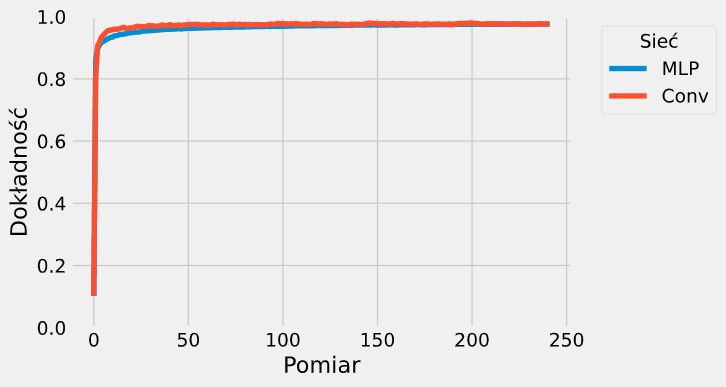
\includegraphics[width=\textwidth]{con_mlp_acc.png}
	\label{fig:res21}
\end{figure}
\begin{figure}[H]
	\centering
	\caption{Porównanie dokładności modeli w końcowym etapie uczenia}
	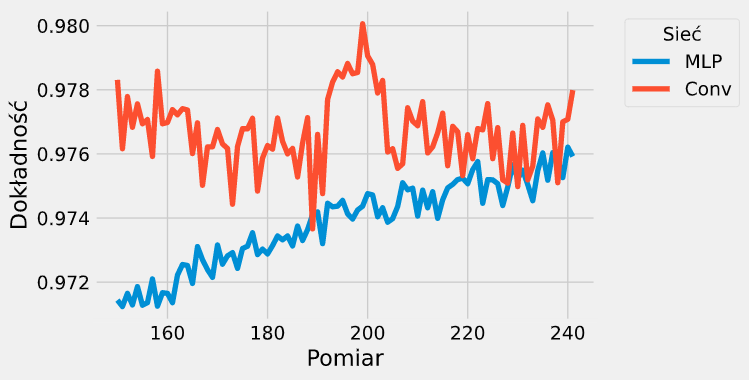
\includegraphics[width=\textwidth]{con_mlp_acc_zoom.png}
	\label{fig:res22}
\end{figure}
\begin{figure}[H]
	\centering
	\caption{Zachowanie funkcji błędu dla modelu MLP}
	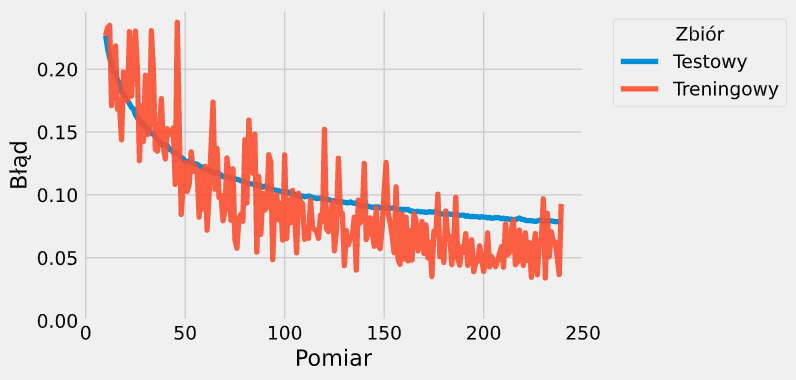
\includegraphics[width=\textwidth]{mlp_err.png}
	\label{fig:res23}
\end{figure}
\begin{figure}[H]
	\centering
	\caption{Zachowanie funkcji błędu dla modelu konwolucyjnego}
	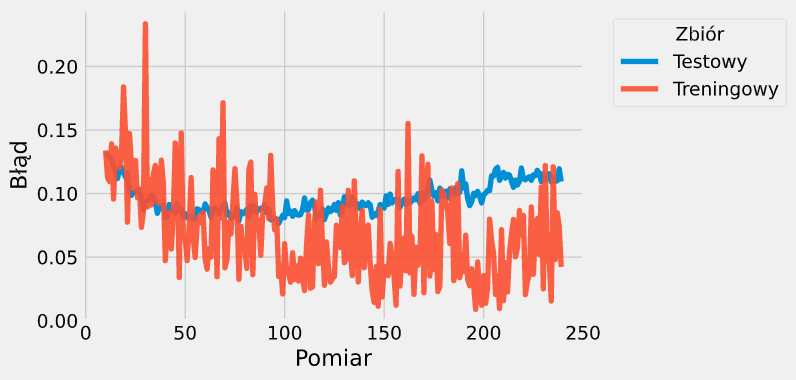
\includegraphics[width=\textwidth]{con_err.png}
	\label{fig:res24}
\end{figure}

\begin{table}[H]
	\caption{Średnia maksymalna dokładność w zależności od modelu}
	\label{tabela-res-21}
	\centering
	\begin{tabular}{rrr}
		\toprule
		Sieć        & Dokładność [\%] \\
		\midrule
		MLP          & 97.73              \\
		Konwolucyjna & \textbf{98.25}     \\
		\bottomrule
	\end{tabular}
\end{table}

\subsubsection*{Wnioski}
Na przedstawionych wykresach~\ref{fig:res21},~\ref{fig:res22} oraz tabeli~\ref{tabela-res-21} widać, że model z warstwą konwolucyjną osiąga lepsze rezultaty od zwykłej sieci MLP. Wpływ na to na pewno ma zdolność konwolucji do wydobywania lokalnych zależności między wartościami, co jest charakterystyczną cechą obrazów. Warstwa konwolucyjna służy jako wstępna ekstrakcja cech przed siecią MLP, co poprawia jej możliwości. Wyraźnie widoczna jest też przewaga sieci splotowej w szybkości osiągnięcia poziomu dokładności bliskiego do ostatecznego. Patrząc jednak na zachowanie funkcji błędu widoczne na wykresach~\ref{fig:res23} i~\ref{fig:res24} można zaobserwować wyraźną tendencję do przeuczenia w przypadku zastosowania konwolucji, w przeciwieństwie do MLP przy którym błąd testowy spada przez cały okres uczenia. Jest to zrozumiałe, jeśli model osiąga dobrą generalizację po zdecydowanie mniejszej ilości przykładów niż MLP to dalsze uczenie go powoduje zbytnie dopasowanie.

\newpage
\section{Wnioski}

\begin{itemize}
	\item Konwolucja idealnie nadaje się do ekstrakcji cech z obrazów, ponieważ wyłapuje lokalne zależności.
	\item Odpowiednia ekstrakcja cech z danych może poprawić skuteczność modelu.
	\item Używanie mniejszych filtrów, wydobywających drobniejsze cechy, może być skuteczniejszym podejściem niż nakładanie dużych i przy tym bardziej kosztownych konwolucji.
	\item Odpowiedni dobór modelu do typu danych skutkuje poprawą wyników.
\end{itemize}

\end{document}